% !TeX root = lfgw.tex
\chapter{Texte schreiben}
\autor{Thomas H. Meyer}

Geistes- und humanwissenschaftliche Arbeiten haben besondere Anforderungen an die typografische
Gestaltung. 
Die häufigsten Anforderungen werden im folgenden der Reihe nach durchgegangen.
Manches davon ist \LaTeX-Standard; anderes wird außerhalb der Geisteswissenschaften eher
selten gebraucht.
Ein großer Bereich, für den \LaTeX{} eigentlich bekannt ist, bleibt ganz außen vor:
der Satz von komplexen mathematischen Formeln und Gleichungen.


\section{Vorüberlegungen zu typographischer Schönheit und Funktionalität}

\dictum[Louis Sullivan]{Form follows function.}

\begin{quote}
 Das Selbermachen ist längst üblich, die Ergebnisse sind oft fragwürdig,
 weil die Laien-Typografen nicht sehen, was nicht stimmt und nicht wissen
 können, worauf es ankommt.
 So gewöhnt man sich an falsche und schlechte Typografie.
 \footcite[9]{erste_hilfe}
 \end{quote}
 
\begin{quotation}
 \emph{Du warst doch mal Sekretärin.
 Ich muß meine Diss schreiben, kannst Du mir zeigen, wie das geht?}
 
 \emph{Was} ein Doktorand oder Diplomand zu schreiben hat, das hat er studiert.
 \emph{Wie} er es zu schreiben hat, hat er nicht studiert, er setzt irgendwie drauflos.
 Mit unübersichtlicher und schlecht lesbarer Laien-Typografie schadet er oft genug seiner Arbeit.
 \footcite[86]{erste_hilfe}
\end{quotation}


Längeres Zitat aus Erste Hilfe Typographie o.\,ä.


\section{Wahl der Dokumentklasse}

In der ersten Zeile eines \LaTeX -Dokumentes wird die Dokumentklasse des folgenden Textes 
festgelegt. Die Dokumentklasse definiert die grundsätzlichen Spielregeln:
Welche Gliederungsebenen sind vorgesehen, wie ist die grundsätzliche Formatierung aufgebaut etc.

Es existiert eine sehr große Vielzahl von verschiedenen Dokumentklassen;
so gibt es für Hausarbeiten oder Dissertationen zahlreicher Universitäten eine eigene
Dokumentklasse. Existiert eine solche, sollte man sie i.\,d.R. auch benutzen.

Die folgende Einführung beschränkt sich auf die Klassen des \KOMAScript-Paketes von
Markus Kohm, weil diese eine überragende typographische Qualität sowie zahllose Möglichkeiten
zur individuellen Anpassung bieten.%
\footnote{Wer allerdings ihre volle Funktionalität nutzen will, sollte sich die originale 
Dokumentation beschaffen und sich mit ihrer Hilfe genauer einarbeiten\dots}
Hinzu treten zwei Dokumentklassen für speziellere Fälle, nämlich für Präsentationen und 
Prüfungen.

\begin{labeling}{scrreprt}
 \item[scrartcl] ist die \KOMAScript-Klasse für Artikel.
 \item[scrreprt] kann gut für längere Seminar- oder auch Bachelor-Arbeiten genutzt werden.
 \item[scrbook] ist die Klasse für Bücher mit zahlreichen ausgereiften Funktionen für
  die Titelei etc.
 \item[exam] ist eine eigene Klasse zur Entwicklung von Aufgabenblättern zu Prüfungszwecken.
 \item[beamer] stellt eine ganze Reihe von features für die Erstellung von Präsentationen
  zur Verfügung. Mit etwas Einarbeitung gelingen damit schneller bessere Präsentationen als 
  mit der verbreiteten Konkurrenz.
\end{labeling}


\minisec{Zum Unterschied zwischen KLASSE und Paket}

Eine \textbf{Dokumentklasse} ...

\textbf{Pakete} ...


\section{Nationale Besonderheiten -- das Paket \paket{babel}}
\label{babel}

\dictum[HPW 104]{Wenn ich nur das Wort Europa höre, entsichere ich meine Dicke Bertha.}

\paket{babel}

Aufruf: \lstinline/\usepackage[<Liste mit benutzen Sprachen>]{babel}/ 

Babel unterstützt eine ganze Reihe von Sprachen; für Geisteswissenschaftler am wichtigsten sind
wohl:

\begin{description}
 \item[german] Deutsch, alte Rechtschreibung (1901)
 \item[ngerman] Deutsch gemäß der Rechtschreibreform von 1996
 \item[greek] Neugriechisch (nur Akut, keine \emph{spiritus}, wahrscheinlich auch kein \emph{Iota subscriptum})
%von Philipp angepaßt, war vorher:
% \item[polutonikogreek] (XXX was ist der Unterschied)
 \item[greek.ancient oder polutonikogreek] Altgriechisch (Akut, Gravis, Zirkumflex; spiritus lenis und asper; Iota subscriptum)
\end{description}

Die als letztes genannte Sprache stellt die Standardsprache des Dokuments (die am Anfang
eingestellt ist) dar.

Auch der Dokumentklasse sollte man die Standardsprache des Dokumentes bekanntgeben.
Denn zahlreiche Pakete , die später geladen werden, werten diese Sprachoption aus und 
passen sich an (z.\,B. \paket{varioref}).

Somit ergibt sich folgender Typische Dokumentbeginn:

\begin{lstlisting}
 \documentclass[ngerman]{scrreprt}
 \usepackage[polutonikogreek,ngerman]{babel}
\end{lstlisting}

\minisec{Wechsel zu einer anderen Sprache}

Im laufenden Dokument kann auf eine der im Paketaufruf angegebenen Sprachen umgeschaltet werden:

\begin{lstlisting} 
 \selectlanguage{polutonikogreek}
\end{lstlisting}



\minisec{Alternative: Das Paket \paket{polyglossia}}

\paket{polyglossia}


\section{Seitengestaltung und Seitenspiegel}
\label{komaskript}
\index{Seitenspiegel} \index{Goldener Schnitt}

Die folgenden Angaben sind nur von Interesse, wenn man als Papierformat nicht Din"~A4-Papier 
nutzen will.

\KOMAScript{}


\minisec{Einstellen des Papierformats}

\paket{geometry}
\index{Papierformat}


\minisec{Beschnittmarken}
\index{Beschnittmarken}
\paket{crop}


\minisec{Ein- oder zweiseitiges Layout}


\section{Textgliederung}

\begin{lstlisting}
 \part{Ein Teil des Teils}
 
 \chapter{Ein Kapitel}
 
 \section{Ein Abschnitt}
 
 \subsection{Ein Unterabschnitt}
 
 \subsubsection{Ein kleiner Unterabschnitt}
 
 \chapter*{Ein Kapitel ohne Eintrag im Inhaltsverzeichnis}
 
 \section*{Ein Abschnitt ohne Eintr. im Inhaltsverz.}
 
 \subsection*{Ein Unterabs. o. E. im Iv.}
 
 \subsubsection*{Ein kleiner Unterabschnitt o.\,E.i.\,I.}
 
 \chapter[Kurzfssg. f. d. Kolumnentitel]{Ein Kapitel}
 
 \section[Kurzfssg. f. d. Kolumnentitel]{Ein Abschnitt}
 
 \subsection[Kurzfssg. f. d. Kolumnentitel]{Ein Unterabschnitt}
\end{lstlisting}

Texte lassen sich in \LaTeX{} m.\,H. eines hierarchischen Systems von Überschriften gliedern:

\begin{description}
 \item[1-9] Texte der Kategorien 
    \lstinline/book/, 
    \lstinline/scrbook/, 
    \lstinline/report/ und 
    \lstinline/scrrprt/ 
 bestehen aus Teilen (\lstinline/\part{}/)
 \footnote{Ehrlich gesagt: eher selten. 
 \lstinline/part/ 
 erzeugt einen sog. \enquote{Zwischentitel},
 der im deutschsprachigen Raum eher unüblich ist. Ausprobieren! }
 und Kapitel (\lstinline/\chapter/);
 desweiteren lassen sich alle Texte in Abschnitte und Unterabschnitte untergliedern 
 (\lstinline/\section{}/ bis \lstinline/\subsubsection{}/) 
 gliedern.
 Jede Überschrift beeinflusst die Kolumnentitel (s.\,u.) und erzeugt automatisch einen Eintrag
 im Inhaltsverzeichnis.
 \item[1-9] Die sog. \enquote{Sternvarianten} der Gliederungsbefehle erzeugen die gleiche
 Formatierung der Überschriften, hinterlassen aber keinen Eintrag im Inhaltsverzeichnis.
 Außerdem werden die Überschriften nicht nummeriert.
 \item[19-23] Die Kapitel und ggf. Abschnittsüberschriften werden auch als lebende Kolumnentitel
 verwendet. Wenn sie dafür zu lang sind, kann man in eckigen Klammern einen alternativen
 Kurztitel zur Verwendung als Kolumnentitel angeben. \index{Kolumnentitel}
\end{description}



\section{Schriftauszeichnungen}
\index{Auzeichnungsschriften}

\dictum[Mies van der Rohe]{Weniger ist mehr.}

\minisec{Auszeichnung über Schriftschnitt}
\index{Schriftschnitt}
\index{kursiv}
\index{Kapitälchen}
\index{fett}
\index{Unterstreichung}

\begin{tabular}{lll}
 \lstinline/\emph{}/ 		&	\emph{hervorgehoben} (z.\,B. kursiv in recte-Texten) 		&	+ \\
 \lstinline/\textit{}/		&	\textsl{kursiv} &	-- -- \\
 \lstinline/\textsl{}/		&	\textsl{schräggestellt} &	-- -- \\
 \lstinline/\textsc{}/		&	\textsc{Kapitälchen}	&	+ \\
 \lstinline/\textbf{}/ 		&	\textbf{fett} 		&	+/- \\
 \lstinline/\underline{}/ 	&	\underline{unterstrichen} &	-- \\
 \lstinline/\texttt{}/		&	\texttt{Schreibmaschinenschrift} &	? \\ 
 \end{tabular} 


\minisec{Veränderung der Schriftgröße}
\index{Schriftgröße}

\begin{tabular}{ll}
 \lstinline/\Huge{}/		&	\Huge{Riesig!} \\
 \lstinline/\huge{}/		&	\Huge{riesig} \\
 \lstinline/\LARGE{}/		&	\LARGE{sehr, sehr groß} \\
 \lstinline/\Large{}/		&	\Large{sehr groß} \\
 \lstinline/\large{}/		&	\large{groß} \\
 \lstinline/\normalsize{}/	&	\normalsize{normal groß (Grundschriftgröße)} \\
 \lstinline/\small{}/		&	\small{klein} \\
 \lstinline/\footnotesize{}/	&	\footnotesize{so groß wie die Fußnoten} \\
 \lstinline/\scriptsize{}/	&	\scriptsize{für Kleingedrucktes} \\
 \lstinline/\tiny{}/		&	\tiny{wirklich winzig} \\
\end{tabular}


\section{Besondere Schriftarten}

Am bequemsten lassen sich in \LaTeX{} Schriften verwenden, für die bereits ein fertiges
Paket existiert, dass lediglich in der Präambel eingebunden werden muss.


\minisec{Alte deutsche Schriften: Fraktur-Schriften}

{\frakfamily
Mit \LaTeX{} lassen sich drei ältere deutsche Schriftarten sehr komfortabel und mit 
professionellem Anspruch verwenden:}

\begin{enumerate}
 \item {\frakfamily Die Frakturschrift, die in Deutschland bis: 1941 die Standardschrift war.
    Sie wirkt sehr feingliedrig, ist gut zu lesen (mit etwas: Übung) und benötigt 
    übrigens: sehr wenig Platz.}
 \item {\gothfamily Die gotische Schrift, die direkt auf Johannes: Gutenberg zurückgeht.}
 \item {\swabfamily Die Schwabacher, die vor allem in der frühen Neuzeit eine sehr weit
    verbreitete Gebrauchsschrift war.}
\end{enumerate}

{\frakfamily
Alle drei Schriftarten werden durch das: Paket}
\paket{yfonts}
{\frakfamily
von Yannis Haralambous: zugänglich gemacht.

(Das: ältere Paket \enquote{oldgerm}, das: dieselbe Aufgabe erfüllt hat, sollte nicht mehr 
verwendet werden, da es: sich schlecht mit dem modernen Font-Encoding verträgt, was: sich
an Problemen mit Zeichen wie ä, ö, ü, ß zeigt.)

Abweichende Schriftschnitte wie kursiv, geneigt oder (halb-)fett stehen nicht zur 
Verfügung.

Doch dabei lauert eine Stolperfalle:
Das: Paket bietet nur die Unterstützung für die Fonts:, das: heißt zahlreiche Erleichterungen
zur Eingabe etc., enthält aber nicht selbst die Fonts:.
Diese müssen separat installiert werden, sonst lässt sich}
\paket{yfonts}
{\frakfamily 
zwar einbinden, doch der Aufruf der Schriften verursacht eine Fehlermeldung und 
statt hübscher Frakturschrift stehen in der PDF-Datei nur leere Flächen.

Das: Paket stellt sechs: Befehle zur Verfügung:}

\begin{itemize}
 \item \lstinline/\frakfamily/
 \item \lstinline/\textfrak{...}/
 \item \lstinline/\gothfamily/
 \item \lstinline/\textgoth{...}/
 \item \lstinline/\swabfamily/
 \item \lstinline/\textswab{...}/
\end{itemize}

{\frakfamily
Der jeweils: erste Befehl stellt die Schrift dauerhaft auf Fraktur, Gotisch oder
Schwabacher um; der jeweils: zweite Befehl dient, um eine kürzere Passage in der 
jeweiligen Schriftart aus:zugeben.}

{\frakfamily 
Typographisch muß man beachten, daß die Frakturschrift zwei Zeichen für das: kleine S hat:
}

\begin{itemize}
 \item \textfrak{s: steht am Wortausgang sowie auch bei zusammengesetzten Wörtern.
  Es: wird als:}
  \lstinline/s:/  
  \textfrak{eingegeben.}
 \item \textfrak{s steht im Wortinneren.}
\end{itemize}

{\frakfamily
Wenn man schon Fraktur-Schrift benutzt, sollte man sich ein wenig aus:kennen und muß
sich in den Schriftcharakter einfühlen. So verträgt sich Fraktur mit der Rechtschreibreform
von 1996 nur sehr schlecht: Wörter wie \enquote{daß} verlangen nach der SZ-Ligatur.
Die Paketdokumentation enthält nicht nur Hinweise zur technischen Benutzung des: 
Paketes:, sondern auch zu gestalterischen Fragen im Zusammenhang mit der Frakturschrift.
}


\minisec{Schreibschriften}
\index{Schreibschrift}

Das Paket \paket{schulschriften} von Walter Entenmann bietet verschiedene deutsche Schulschriften.
\footcite[Zur Geschichte der deutschen Schulschriften sowie dem Vorgehen zu ihrer Implementierung 
in \LaTeX:][]{entenmann:dtk2012/4}

Zu beachten ist, dass das Paket nicht mit \lstinline/\usepackage/ eingebunden werden muss;
das ist auch nicht möglich, da es keine Paketdatei (\enquote{schulschriften.sty}) anbietet.
Es reicht aus, die Fontdateien zu installieren.

Die Fonts müssen dann über den eigentlichen Fontauswahlmechanismus von \LaTeXe{} angesprochen werden:

Sütterlin-Schrift mit gerader Feder:

\begin{LTXexample}
{\usefont{T1}{wesu}{m}{n}
\huge
Ich kann schreiben!}
\end{LTXexample}

Sütterlin-Schrift geneigt mit Bandzugfeder:

\begin{LTXexample}
{\usefont{T1}{wesu}{b}{sl}
\huge
Ich kann schreiben!}
\end{LTXexample}


Deutsche Normalschrift:

\begin{LTXexample}
{\usefont{T1}{wedn}{m}{sl}
\huge
Ich kann schreiben!}
\end{LTXexample}

Lateinische Ausgangsschrift:

\begin{LTXexample}
{\usefont{T1}{wela}{m}{sl}
\huge
Ich kann schreiben!}
\end{LTXexample}

Schulausgangsschrift:

\begin{LTXexample}
{\usefont{T1}{wesa}{m}{sl}
\huge
Ich kann schreiben!}
\end{LTXexample}

Vereinfachte Ausgangsschrift:

\begin{LTXexample}
{\usefont{T1}{weva}{m}{sl}
\huge
Ich kann schreiben!}
\end{LTXexample}

Die ausgezeichnete deutschsprachige Paketdokumentation eignet sich übrigens sehr gut,
den dahinterliegenden Fontauswahlmechanismus von \LaTeX{} kennenzulernen.

In der Praxis wird man die Fontaufrufe in ein selbstdefiniertes Makro verpacken, 
vgl. \ref{makros} auf S.~\pageref{makros}.


\section{Sonderzeichen}

\cite{voss:dtk20011/1}

\minisec{Der Wortzwischenraum}

Der übliche Wortzwischenraum (Fachbezeichnung: Spatium (NEIN, das Spatium ist nur eine Ergänzungmöglichkeit. Heute bei LaTeX als \, bekannt)) wird von \LaTeX{} beim Absatzumbruch innerhalb einer Zeile
gleichmäßig verteilt. Die Eingabe erfolgt in Form von normalen Leerzeichen oder als 
einfacher Zeilenwechsel.

Folgende beiden Eingaben sind also gleichwertig:

\begin{LTXexample}
 superbia avaritia invidia ZORN UNKEUSCHHEIT UNMAESSIGKEIT acedia
 
 Wort1
 Wort2
 Wort3
 Wort4
 Wort5
 Wort6
 Wort7
\end{LTXexample}

Ein sog. \enquote{fester Ausschuss} ist in der Setzersprache ein Wortzwischenraum, an dem 
kein Zeilenwechsel durchgeführt werden darf. Er wird mit dem Zeichen \lstinline/~/
codiert:

\begin{LTXexample}
 Kunst und Kultur im 19.~Jahrhundert
\end{LTXexample}

Manchmal ist es nötig, an einzelnen Stellen längere Spatien zu werden, etwa um Halbverse 
in epischen Dichtungen zu markieren. Dazu kann man mehrere feste Ausschüsse verbinden:

\begin{lstlisting}
 \begin{verse}
 Uns ist in alten maeren ~ wunders vil geseit\\
 von heleden lobebaeren ~ von von grozer arebeit\\
 von fröuden, hochgeziten, ~ von weinen und von klagen,\\
 von küener recken striten ~ muget ir nu wunders hoeren sagen.
 \end{verse}
\end{lstlisting}

Daraus wird:

 \begin{verse}
 Uns ist in alten maeren ~ wunders vil geseit\\
 von heleden lobebaeren ~ von von grozer arebeit\\
 von fröuden, hochgeziten, ~ von weinen und von klagen,\\
 von küener recken striten ~ muget ir nu wunders hoeren sagen.
 \end{verse}


\minisec{Leerzeichen vermeiden -- das Zeichen \%}

\LaTeX{} hält sich bekanntlich nicht an die Zeilenaufteilung der Quelldatei. Erst eine Leerzeile
wird als Absatzgrenze interpretiert. Einfache Zeilenwechsel führen zu einem normalen 
Wortzwischenraum. Dies kann unerwünscht sein:

Besonders bei komplexeren \LaTeX -Strukturen kann es sinnvoll sein, Zeilenwechsel einzufügen,
z.\,B. zwischen einzelnen Befehlen oder einem Wort und einer folgenden Fußnote.
An diesen Stellen soll aber kein Wortzischenraum -- womöglich sogar ein sich ergebender 
Zeilenwechsel -- eingefügt werden.

Dazu kann man das Kommentarzeichen \% an das Zeilenende setzen. Der Zeilenwechsel wird auf diese 
Weise quasi \enquote{auskommentiert}, bei der Übersetzung des Dokuments mit \LaTeX\
verschwindet er vollständig.

Man beachte den Unterschied:

\begin{LTXexample}
 Wort1
 Wort2
 
 Wort3%
 Wort4
\end{LTXexample}


\minisec{Sonderzeichen für Germanisten}

Quasi unterhalb der Ebene von Unicode mit seinem Zugang zum gesamten Zeichensatz hält 
\LaTeX{} einige Sonderzeichen bereit, die z.\,B. für Germanisten von besonderem Interesse
sein dürften. Sie können als besondere Befehle eingegeben werden:

\begin{tabular}{ll}
 kleines \th & 	\lstinline/\th/ \\
 großes \TH & 	\lstinline/\TH/ \\
\end{tabular}
\index{Thorn}

Lädt man zusätzlich das \paket{textcomp}, stehen eine ganze Reihe weiterer Symbole
zur Verfügung:

\begin{tabular}{ll}
 \pounds & 	\lstinline/\pounds/ \\
 \copyright & 	\lstinline/\copyright/ \\
 \texteuro & 	\lstinline/\texteuro/ \\
 \textborn & 	\lstinline/\textborn/ \\
 \textmarried & 	\lstinline/\textmarried/ \\
 \textdied & 	\lstinline/\textdied/ \\
 \end{tabular}
 
Dies stellt nur eine winzige Teilmenge der in \LaTeX{} zur Verfügung stehenden Sonderzeichen dar;
eine vollständige Übersicht bietet die \enquote{Comprehensive \LaTeX{} Symbol List} von
Scott Pakin (331 Seiten, Stand Nov. 2015).
\footnote{\lstinline/texdoc comprehensive/}


\minisec{Akzenze und Diakritika}

Diakritika \index{Diakritika},
Betonungszeichen etc.


\minisec{Unicode-Codes}

Was immer geht: 
vgl. Abschnitt \ref{unicodeeingabe} auf S.~\pageref{unicodeeingabe} 
(für die Eingabemethode)
bzw. Abschnitt \ref{utf8codes} auf S.~\pageref{utf8codes} 
(für eine Übersicht über häufig benötigte Unicode-Zeichen und ihre Codes).


\minisec{Einzelne griechische Buchstaben}
\label{griechEinzelbuchstaben}

Das Paket \paket{textgreek} erlaubt die einfache Eingabe griechischer Buchstaben.
Es ist natürlich weniger geeignet, ganze Texte auf Griechisch zu erfassen, kann aber sehr
praktisch sein, wenn es eben nur um wenige einzelne Zeichen geht:

\begin{center}
\begin{tabular}{llll}
 \textalpha & 	\lstinline/\textalpha/ &	\textAlpha &	\lstinline/\textAlpha/ \\
 \textbeta & 	\lstinline/\textbeta/ &		\textBeta &	\lstinline/\textBeta/ \\
 \textgamma & 	\lstinline/\textgamma/ &	\textGamma &	\lstinline/\textGamma/ \\
 \textdelta & 	\lstinline/\textdelta/ &	\textDelta &	\lstinline/\textDelta/ \\
 \textepsilon & \lstinline/\textepsilon/ &	\textEpsilon &	\lstinline/\textEpsilon/ \\
 \textzeta & 	\lstinline/\textzeta/ &		\textZeta &	\lstinline/\textZeta/ \\
 \texteta & 	\lstinline/\texteta/ &		\textEta &	\lstinline/\textEta/ \\
 \texttheta & 	\lstinline/\texttheta/ &	\textTheta &	\lstinline/\textTheta/ \\
 \textiota & 	\lstinline/\textiota/ &		\textIota &	\lstinline/\textIota/ \\
 \textkappa & 	\lstinline/\textkappa/ &	\textKappa &	\lstinline/\textKappa/ \\
 \textlambda & 	\lstinline/\textlambda/ &	\textLambda &	\lstinline/\textLambda/ \\
 \textmu & 	\lstinline/\textmu/ &		\textMu &	\lstinline/\textMu/ \\
 \textnu & 	\lstinline/\textnu/ &		\textNu &	\lstinline/\textNu/ \\
 \textxi & 	\lstinline/\textxi/ &		\textXi &	\lstinline/\textXi/ \\
 \textomikron & \lstinline/\textomikron/ &	\textOmikron &	\lstinline/\textOmikron/ \\
 \textpi & 	\lstinline/\textpi/ &		\textPi &	\lstinline/\textPi/ \\
 \textrho & 	\lstinline/\textrho/ &		\textRho &	\lstinline/\textRho/ \\
 \textsigma & 	\lstinline/\textsigma/ &	\textSigma &	\lstinline/\textSigma/ \\
 \texttau & 	\lstinline/\texttau/ &		\textTau &	\lstinline/\textTau/ \\
 \textupsilon & \lstinline/\textupsilon/ & 	\textUpsilon &	\lstinline/\textUpsilon/ \\
 \textphi & 	\lstinline/\textphi/ &		\textPhi &	\lstinline/\textPhi/ \\
 \textchi & 	\lstinline/\textchi/ &		\textChi &	\lstinline/\textChi/ \\
 \textpsi & 	\lstinline/\textpsi/ &		\textPsi &	\lstinline/\textPsi/ \\
 \textomega & 	\lstinline/\textomega/ &	\textOmega &	\lstinline/\textOmega/ \\
\end{tabular}
\end{center}

Offene Frage: Akzente

Wo liegt die Schmerzgrenze für dieses Verfahren?
Wahrscheinlich bei etwas über einem Wort...

Comprehensive S.~


\minisec{Ein \enquote{kleines Ärgernis}: Anführungszeichen}
\label{enquote}

Nicht einfach die Gänsefüßchen \lstinline/"/ benutzen, das diese nicht korrekt interpretiert
werden können: Es ist für den Computer schwer erkennbar, wo die Anführung beginnt und wo sie
endet. Entsprechende regelbasierte Automatiken sind notorisch fehleranfällig.
Da die zugrundeliegenden Regeln nicht ganz trivial sind,
\footnote{Lesetypographie seite ...}
kommen -- auch in professionell gesetzten Büchern häufig Fehler vor.
Man sollte daher möglichst auf eine händische Eingabe ganz verzichten.

Am sinnvollsten ist der Weg, das Paket \paket{csquotes} einzubinden (in der Präambel) und auf 
eine manuelle Eingabe der Anführungszeichen ganz zu verzichten: Statt dessen definiert das Paket
ein Makro namens \lstinline/\enquote{}/, das als Ersatz für die Anführungszeichen eingegeben
wird.

Das Paket erkennt, welche Sprache für das Dokument (mittels \paket{babel} oder \paket{polyglossia})
eingestellt worden ist, und ersetzt die codierung \lstinline/\enquote{}/ durch die 
jeweils korrekte Form -- auch bei geschachtelt auftretenden Anführungszeichen:

\begin{LTXexample}
Er sprach: \enquote{Hast du den \enquote{Faust} gelesen?} 

\selectlanguage{french}
Er sprach: \enquote{Hast du den \enquote{Faust} gelesen?} 

\selectlanguage{english}
He asked, \enquote{Have you read \enquote{On The Road} yet?} 
\end{LTXexample}

Die Verwendung von \paket{csquotes} hat noch einen zweiten Vorteil:
Man kann an einer Stelle, nämlich bei den Optionen des Paketes, auch andere Anführungszeichen 
einstellen und muss nicht alle einzelnen Stellen umcodieren.

Arbeitsumgebungen wie kile lassen sich übrigens so einstellen, dass die Eingabe von Shift + 2
automatisch \lstinline/\enquote{/ oder \lstinline/}/ erzeugt.


rotatebox

reflectbox


\section{Listen und Aufzählungen}

\LaTeX{} bietet eine ganze Reihe von Möglichkeiten, Listen und Aufzählungen zu gestalten.
Hier werden nur die grundlegenden Funktionen gezeigt; daneben gibt zahlreiche Möglichkeiten zur
Modifikation.\footcite[295\psqq]{voss:einfuehrung}

%Philipp schlägt vor, compactenum vorzustellen!

\minisec{\enquote{Triviale} Listen ohne alles: trivlist}

Am anspruchlosesten ist die einfache Auflistung ohne irgendwelche Formatierung:

\begin{LTXexample}
\begin{trivlist}
 \item der erste Punkt,
 \item der zweite Punkt,
 \item der dritte Punkt.
\end{trivlist} 
\end{LTXexample}


\minisec{\enquote{Normale} Liste mit Aufzählungszeichen: itemize}

\begin{LTXexample}
\begin{itemize}
 \item der erste Punkt,
 \item der zweite Punkt,
 \item der dritte Punkt.
\end{itemize} 
\end{LTXexample}

XXX Erklären: Verändern des Aufzählungszeichens für einen einzelnen Punkt und generell.


\minisec{Durchnumerierte Aufzählung: enumerate}

\begin{LTXexample}
\begin{enumerate}
 \item der erste Punkt,
 \item der zweite Punkt,
 \item der dritte Punkt.
\end{enumerate} 
\end{LTXexample}

Durch Verändern des Zählers \lstinline/enumi/ kann man den Startpunkt der 
Aufzählung verändern:

\begin{LTXexample}
\begin{enumerate}
 \setcounter{enumi}{123}
 \item der erste Punkt,
 \item der zweite Punkt,
 \item der dritte Punkt.
\end{enumerate} 
\end{LTXexample}


\minisec{Erweiterte Möglichkeiten: das Paket \paket{enumitem}}

Nur darauf hingewiesen sei auf das Paket \paket{enumitem}, mit dem sich zahlreiche 
weitere Sonderwünsche verwirklichen lassen.\footcite[304\psqq]{voss:einfuehrung}
Die Umgebung \lstinline/enumerate/  kann dahingehend modifiziert werden, sodass es ebenso möglich ist, 
die durchnummerierten Label selbst zu definieren
und auf diese im Fließtext zu verweisen:

\begin{example}
\begin{enumerate}[%
  label={\bfseries \arabic{*}. Fall:\ },
  ref={\arabic{*}. Fall}]
\item Nominativ \label{fall:1}
\item Genitiv\label{fall:2}
\item Dativ\label{fall:3}
\item Akkusativ\label{fall:4}
\end{enumerate}
Der \ref{fall:1} wird auch Werfall gennant,
der \ref{fall:4} hingegen Wenfall.
\end{example}

\begin{description}
 \item[2] Modifikation des Zählers: 
 Mit \lstinline/label=/ wird definiert,
 wie der Zähler beschriftet ist; hier wird er fett gesetzt und 
 erhält eine arabische Nummer an die als Ergänzung \enquote*{. Fall:} gesetzt wird.
  \item[3] Modifikation der Referenz: 
   Mit \lstinline/ref=/ wird definiert,
   wie beim Aufruf von \lstinline/\ref/ der Verweis aussehen soll;
   hier wie das Label jedoch ohne Fettung. 
 \end{description}
 \iffalse
 \begin{enumerate}[%
  label={\bfseries \arabic{*}. Fall:\ },
  ref={\arabic{*}. Fall}]
\item Nominativ \label{fall:1}
\item Genitiv\label{fall:2}
\item Dativ\label{fall:3}
\item Akkusativ\label{fall:4}
\end{enumerate}
Der \ref{fall:1} wird auch Werfall gennant,
der \ref{fall:4} hingegen Wenfall.
 \fi
\minisec{Worterklärung, Glossar I: description}
\index{Glossar}

Besonders für Worterklärungen o.\,ä. eignet sich die Umgebung \lstinline/description/,
die zu jedem \lstinline/\item/  eine Angabe in eckigen Klammern erwartet:

\begin{LTXexample}
\begin{description}
 \item[AT] das Alte Testament
 \item[NT] das Neue Testament 
\end{description} 
\end{LTXexample}


\minisec{Worterklärung, Glossar II: labeling}
Die Dokumentklassen von \KOMAScript\ stellen eine weitere Umgebung bereit, die die 
Formatierung von Schlagwortlisten noch weiter verfeinert:

\begin{lstlisting}
 \begin{labeling}[Trennzeichen]{Musterlänge}
  \item[Schlagwort] Text
 \end{labeling}
\end{lstlisting}

Das Trennzeichen steht zwischen den Schlagwörtern und der Erklärung und die Musterlänge definiert
die Breite der linken Spalte:

\begin{LTXexample}
 \begin{labeling}[=]{NSDAP}
  \item[DDP] Deutsche Demokratische Partei
  \item[DNVP] Deutschnationale Volkspartei
  \item[DVP] Deutsche Volkspartei
  \item[NSDAP] Nationalszozialistische Deutsche Arbeiterpartei
  \item[SPD] Sozialdemokratische Partei Deutschlands
 \end{labeling}
\end{LTXexample}

Wie alle Teile von \KOMAScript\ gibt es zahlreiche Möglichkeiten, die Gestaltung zu
beeiflussen. Um diese Möglichkeiten auszuschöpfen, muss man sich mit der Dokumentation 
beschäftigen.


\minisec{Geschachtelte Listen}

Ein besonderer Reiz besteht darin, dass ich die verschiedenen Listenumgebungen praktisch
beliebig komplex verschachteln lassen:

\begin{LTXexample}
\begin{itemize}
 \item Sieben freie Künste:
 \begin{itemize}
   \item Trivium:
   \begin{itemize}
    \item Grammatik
    \item Logik
    \item Rhetorik
   \end{itemize}
   \item Quadrivium:
   \begin{itemize}
    \item Arithemtik
    \item Geometrie
    \item Astronomie
    \item Musik
   \end{itemize}
 \end{itemize}
 \item Höhere Fakultäten:
 \begin{itemize}
   \item Theologie
   \item Medizin
   \item Jura
 \end{itemize}
\end{itemize}
\end{LTXexample}




\section{Textpassagen zitieren}

\minisec{Zitate im Fließtext}

Normale Eingabe;
Anführungszeichen am besten mit \lstinline/\enquote{}/ codieren (vgl. S.~\pageref{enquote}); 
Textstellen belegen mit Fußnote und automatischer Literaturverwaltung.


\minisec{\enquote{Schlauer Spruch} am Kapitelanfang}
\dictum[Sinnspruch nach Boethius]{Si tacuisses, philosophus mansisses.}

\enquote{Ein häufiger anzutreffendes Element ist ein Zitat oder eine Redewendung, die rechtsbündig unter 
oder über einer Überschrift gesetzt wird. dabei werden der Spruch selbst und der Quellennachweis
in der Regel speziell formatiert.}\footcite[131]{kohm:2014}

\KOMAScript\ stellt hierfür den Befehl \lstinline/\dictum[Urheber]{Spruch}/ zur Verfügung.

Die angesprochene Formatierung lässt sich in allen Details verändern.
\footcite[vgl.][131\psqq]{kohm:2014}


\minisec{Einen Abschnitt zitieren: quote}

Die Umgebung \lstinline/quote/ eignet sich dazu, ein Zitat von der Länge eines Absatzes einzubauen:

\begin{quote}
 Seit Anfang März wusste der Diktator, dass die Tage der Diktatur gezählt waren.
\end{quote}

(Der Beginn der Kurzgeschichte \enquote{Cäsar und sein Legionär} von Bertolt Brecht.)


\minisec{Eine längere Passage zitieren: quotation}

Soll das gewünschte Zitat etwas länger ausfallen, wählt man statt dessen besser die 
Umgebung \lstinline/quotation/:

\begin{LTXexample}
\usepackage[utf8]{inputenc}
\usepackage[T1]{fontenc}

Die Kurzgeschichte \enquote{Cäsar und sein Legionär} von B. Brecht beginnt so:

\begin{quote}
 Seit Anfang März wusste der Diktator, dass die Tage der Diktatur gezählt waren.

 Ein Fremder, aus einer der Provinzen kommend, hätte die Hauptstadt vielleicht imposanter
 denn je gefunden... 
\end{quote}
\end{LTXexample}

\minisec{Ein Gedicht zitieren: verse}
\index{Gedicht} \index{Lyrik}

Das standardmäßige Umgebung \lstinline/verse/ erlaubt mit sehr wenig Mühe den Einbau von 
Gedichtpassagen, allerdings auch mit ziemlich einfacher Typografie:

\begin{LTXexample}
\minisec{Der Lorscher Bienensegen:}
\begin{verse}
 Kirst, imbi ist hucze! \\
 nu fluic du, uihi minaz, hera \\
 fridu frono in godes munt \\
 heim zi commone gisunt. \\
 sizi, sizi, bina: \\
 inbot dir sancte maria. \\
 hurulob ni habe du: \\
 zi holce ni fluc du, \\
 noh du mir nindrinnes, \\
 noh du mir nintuuinnest. \\
 sizi uilu stillo, \\
 vuirki godes uuillon.
\end{verse}
\end{LTXexample}

Strophenzwischenräume

Paket \paket{verse}? wann?

und ab wann \paket{poemscol}?


\minisec{Fremdsprachige Zitate}

Leider nur für polyglossia\footcite[33\psqq]{rouquette:2012}

%Philipp meint: Wo ist das Problem, es geht doch bei Babel auch? \foreignlanguage{sprache}{text}

\section{Fußnoten}

Fußnoten haben eine doppelte Funktion: 
Zum einen können bestimmte Informationen, die den Lesefluss des Haupttextes eher behindern,
Anmerkungen, Erklärungen, Ergänzungen oder Korrekturen in Fußnoten verlagert werden.
Zum anderen dienen -- v.\,a. in den Geisteswissebschaften -- Fußnoten zur Aufnahme der 
Literaturnachweise.

Diese Doppelfunktion spiegelt sich in \LaTeX{} wider, das zwei Befehle zur Fußnotenerstellung
anbietet:

\lstinline/\footnote{...}/ erzeugt eine \enquote{normale}, frei formulierte Fußnote.

\lstinline/\footcite[vordere Ergänzung][hintere Ergänzung]{bibl. Kennung}/ dient dazu,
einen Literaturverweis zu setzen. Die verwendete bibliographische Kennung muss in einer
Bibliografie-Datei aufgeschlüsselt werden und wird vom Programmsystem gemäß den Vorgaben
des eingestellten Bibliografiestils aufgelöst. Dabei lassen sich alle Rafinessen 
humanwissenschaftlicher Fußnotenkunst realisieren. 
Die Details hierzu findet man in Kapitel \ref{biblatex} auf S.~\pageref{biblatex}. 

Nach den Setzerregeln steht die Fußnotenziffer ohne Leerzeichen direkt hinter dem letzten
Satzzeichen oder Wort, auf das sich die Fußnote bezieht.
Wenn der Fußnotenaufruf -- was sehr empfehlenswert ist, um die Quelldatei gut les- und 
verarbeitbar zu halten -- die Fußnote in einer eigenen Zeile steht, sollte man durch ein 
\% -Zeichen die Umwandlung des Zeilenwechsels in ein Leerzeichen verhindern:

\begin{lstlisting}
 Hier steht ein Text%
 \footnote{lat. textus = Gewebe}
 mit Fußnoten.
\end{lstlisting}


\minisec{Fußnotenlayout mit \KOMAScript}

Verwendet man eine \KOMAScript -Klasse, so lassen sich die Fußnoten sehr leicht und vielfältig
den eigenen gestalterischen Wünschen anpassen. Dazu dienen die beiden Befehle
\lstinline/\deffootnote[Markenbreite]{Einzug}{Absatzeinzug}{Markendefinition}/
und 
\lstinline/\deffootnotemark{Markendefinition}/.

Folgende Umdefinitionen erzeugen z.\,B. Fußnoten mit eingeklammerten Ziffern 
in Grundschriftgröße; die jeweils erste Zeile jeder Fußnote ist eingerückt:

\begin{lstlisting}
 \deffootnote[10mm]{0mm}{0mm}{(\thefootnotemark)}
\end{lstlisting}


\minisec{Das Paket \paket{footmisc}}

Das Paket \paket{footmisc} von Robin Fairbains erlaubt zahlreiche Sonderfunktionen, die 
lediglich per Paketoption angewähl werden müssen.

Die m.\,E. nützlichsten Optionen sind:

\begin{description}
 \item[perpage] Die Fußnoten werden seitenweise gezählt. (2 Durchläufe nötig!)
 \item[para] Die Fußnoten werden alle zu einem Absatz zusammengefasst, das spart v.\,a. dann
  viel Platz und verbessert das Druckbild, wenn es sich um sehr kurze Fußnotentexte (etwa nur
  Bibelstellenangaben o.\,ä.) handelt.
 \item[ragged] Die Fußnoten werden im Flattersatz gesetzt.
 \item[hang] Hängender Einzug der Fußnoten (wie in diesem Buch).
  Die Breite des Einzugs wird durch \lstinline/\footnotemargin/ festgelegt.\\
  Achtung: Die Anweisung \lstinline/\setlength{\footnotemargin}{4mm}/ muss \emph{nach}
  \lstinline/\begin{document}/ stehen, der Paketaufruf aber natürlich davor!
 \item[norule] Weglassen der Fußnotenlinie.
 \item[multiple] Wenn mehrere Fußnoten direkt hintereinander stehen, wird zwischen die
  Fußnotenkennungen der Inhalt von \lstinline/\multifootsep/ eingefügt. voreingestellt ist
  ein Komma.
\end{description}



\minisec{Zweispaltige Fußnoten}

Paket ...


\minisec{Mehrere Fußnotenapparate: das Paket \paket{manyfoot}}

%Philipp meint: hier würde ich nur nach hinten auf reledmac verweisen, denn manyfoot verträgt sich bestimmt nicht mit reledmac; und hinten werden dann die Details eh alle schon erklärt.

Das Paket \paket{manyfoot} von Alexander I. Rozhenko
erlaubt die Definition verschiedener Fußnotenapparate, um beispielsweise
Worterklärungen (Fußnoten 1, 2, 3, \ldots ) und Quellenhinweise (a, b, c, \ldots ) voneinander zu trennen.

Auch Lesartenapparate in kritischen Editionsprojekten ließen sich theoretisch 
mit diesem Ansatz organisieren; 
allerdings bietet \paket{reledmac} hierzu die besseren Instrumente, vgl. hierzu \ref{reledmac}.

\section{Zeilennummern} 
\index{Zeilennummern}
\paket{lineno}
\label{zeilennummer}

Es gibt zwei grundsätzlich verschiedene Szenarien, in denen man Zeilennummern verwenden
kann. 

\begin{itemize}
 \item Einfach einen Text(abschnitt) durchnumerieren, z.\,B. auf einem Arbeitsblatt oder in
 einem Lehrbuch.
 \item einen Text mit Zeilennummern versehen, auf die später Bezug genommen wird, 
 z.\,B. im Rahmen einer großen Textausgabe. 
\end{itemize}

Hier wird nur das erste gezeigt;
Aufgabe Nr. 2 ist viel komplexer, s. Kapitel zum Erstellen einer kritischen Edition, 
S.~\pageref{reledmac} 

Das Paket \paket{lineno} bietet eine Reihe von Funktionen, einen Text -- oder 
zahlreiche eingeschobene Texte wie Zitate o.\,ä. mit Zeilennummern als Lesehilfe zu 
versehen.


\minisec{Einen einzelnen Textabschnitt mit Zeilennummern versehen}

Wenn das Paket \paket{lineno} in der Präambel geladen worden ist, kann man im
Dokument durch den Befehl \lstinline/\linenumbers/ die Zeilennummern anschalten.
Durch \lstinline/\nolinenumbers/ wird die Nummerierung wieder abgestellt.
Auch das Ende der aktuellen Umgebung beendet die Zeilennummern.

\begin{lstlisting}
 Georg Büchners \enquote{Lenz} beginnt mit einm langen Textabschnitt:
 
 \begin{quotation}
 \modulolinenumbers[5]
 \linenumbers
 Den 20. ging Lenz durchs Gebirg. Die Gipfel und hohen Bergflächen im Schnee, die Täler
 hinunter graues Gestein...
 \end{quotation}
\end{lstlisting}

Daraus wird:
\bigskip

 Georg Büchners \enquote{Lenz} beginnt mit einem langen Textabschnitt:

 \begin{quotation}
 \modulolinenumbers[5]
 \linenumbers
 Den 20. ging Lenz durchs Gebirg. Die Gipfel und hohen Bergflächen im Schnee, die Täler
 hinunter graues Gestein, grüne Flächen, Felsen und Tannen. Es war naßkalt, das Wasser
 rieselte die Felsen hinunter und sprang über den Weg. Die Äste der Tannen hingen schwer
 herab in die feuchte Luft. Am Himmel zogen graue Wolken, aber alles so dicht, und dann 
 dampfte der Nebel herauf und strich schwer und feucht durch das Gesträuch, so träg,
 so plump. Er ging gleichgültig weiter, es lag ihm nichts am Weg, bald auf- bald
 abwärts. Müdigkeit spürte er keine, nur war es ihm manchmal unangenehm, daß er nicht
 auf dem Kopf gehen konnte.
 \end{quotation}

\minisec{Einstellmöglichkeiten von \paket{lineno}}

Das Paket bietet zahlreiche Möglichkeiten, das Erscheinungsbild der Zeilennummern zu 
verändern:

Beim Aufruf des Paketes können folgende Optionen angegeben werden:

\begin{labeling}{pagewise}
 \item[left] Die Zeilennummern stehen am linken Rand.
 \item[right] Die Zeilennummern stehen am rechten Rand.
 \item[switch] Die Zeilennummern stehen (bei zweiseitigem Layout) am äußeren Rand.
 \item[switch*] Die Zeilennummern stehen am inneren Rand.
 \item[pagewise] Die Zeilennummerierung beginnt auf jeder neuen Seite wieder bei 1.
 \item[modulo] Nur jede x-te Zeile erhält eine Nummer. 
  Das Einstellen der Schrittweite erfolgt durch \cs{modulolinenumbers\oarg{Integer}} 
  (sic! Die Klammern müssen eckig sein...);
  voreingestellt ist der Wert von 5.
\end{labeling}

Makro \cs{linenumberfont} für die Schriftart der Zeilennummer.

Länge \cs{linenumbersep} bestimmt Abstand zwischen Zeilennummer und Text.

Zeilennummern bei größeren Projekten, insbesondere im Kontext von kritischen Editionsprojekten,
sollten mit dem Paket \paket{reledmac} erzeugt werden, vgl. hierzu \ref{reledmac}.

 

\minisec{Eingeschobene Gedichte o.\,ä. mit Zeilennummern}

Auch die Nummerierung eines Gedichtes gelingt auf diese Weise ohne Probleme:

\begin{LTXexample}
 \begin{verse}
  \modulolinenumbers[5]
  \linenumbers
  Ist Liebe lauter nichts,\\
  wie dass sie mich entzündet.\\
  Ist sie dann gleichwohl was,\\
  wem ist ihr tun bewusst?\\
  
  Im Sommer ...\\
 \end{verse}

\end{LTXexample}



\section{Randbemerkungen (Marginalien)}
\index{Randbemerkung}
\index{Marginalien}

Mit dem Befehl \lstinline/\marginpar[links]{rechts}/ kann eine Randbemerkung gesetzt werden.
\marginpar{Randbemerkung}
Dabei ist die Bezeichnung \enquote{links} und \enquote{rechts} missverständlich: 
Randbemerkungen stehen immer außen auf den Seitenrändern; bei zweispaltigem Layout wird 
\emph{auf linken Seiten} der als \lstinline/[links]/ definierte Text ausgegeben, falls vorhanden.

Mit dem Befehl \cs{reversemarginpar} lässt sich dieses Verhalten umkehren; 
von der Benutzung ist abzuraten, da innen stehende Marginalien i.\,d.R. wegen der Bindung schlecht
lesbar sind.

Marginalien, die mit dem \LaTeX -Standardbefehl gesetzt sind, dürfen nicht in Gleitumgebungen
stehen und können selbst nur einfachen Text enthalten.


\minisec{Erweiterte Möglichkeiten für Marginalien}
Das Paket \paket{marginnote} stellt eine verbesserte Variante von Marginalien bereit, 
da marginpar Probleme mit Floats hat:
\cs{marginnote}\oarg{left}\marg{right}\oarg{voffset}
%Beschreibung der Optionen?

Das Paket \paket{sidenotes} von Andy Thomas bietet weitere Möglichkeiten: 
Es ist mit ihm auch möglich, Randbemerkungen innerhalb von Gleitumgebungen zu setzen oder
Bilder
\begin{marginfigure}
 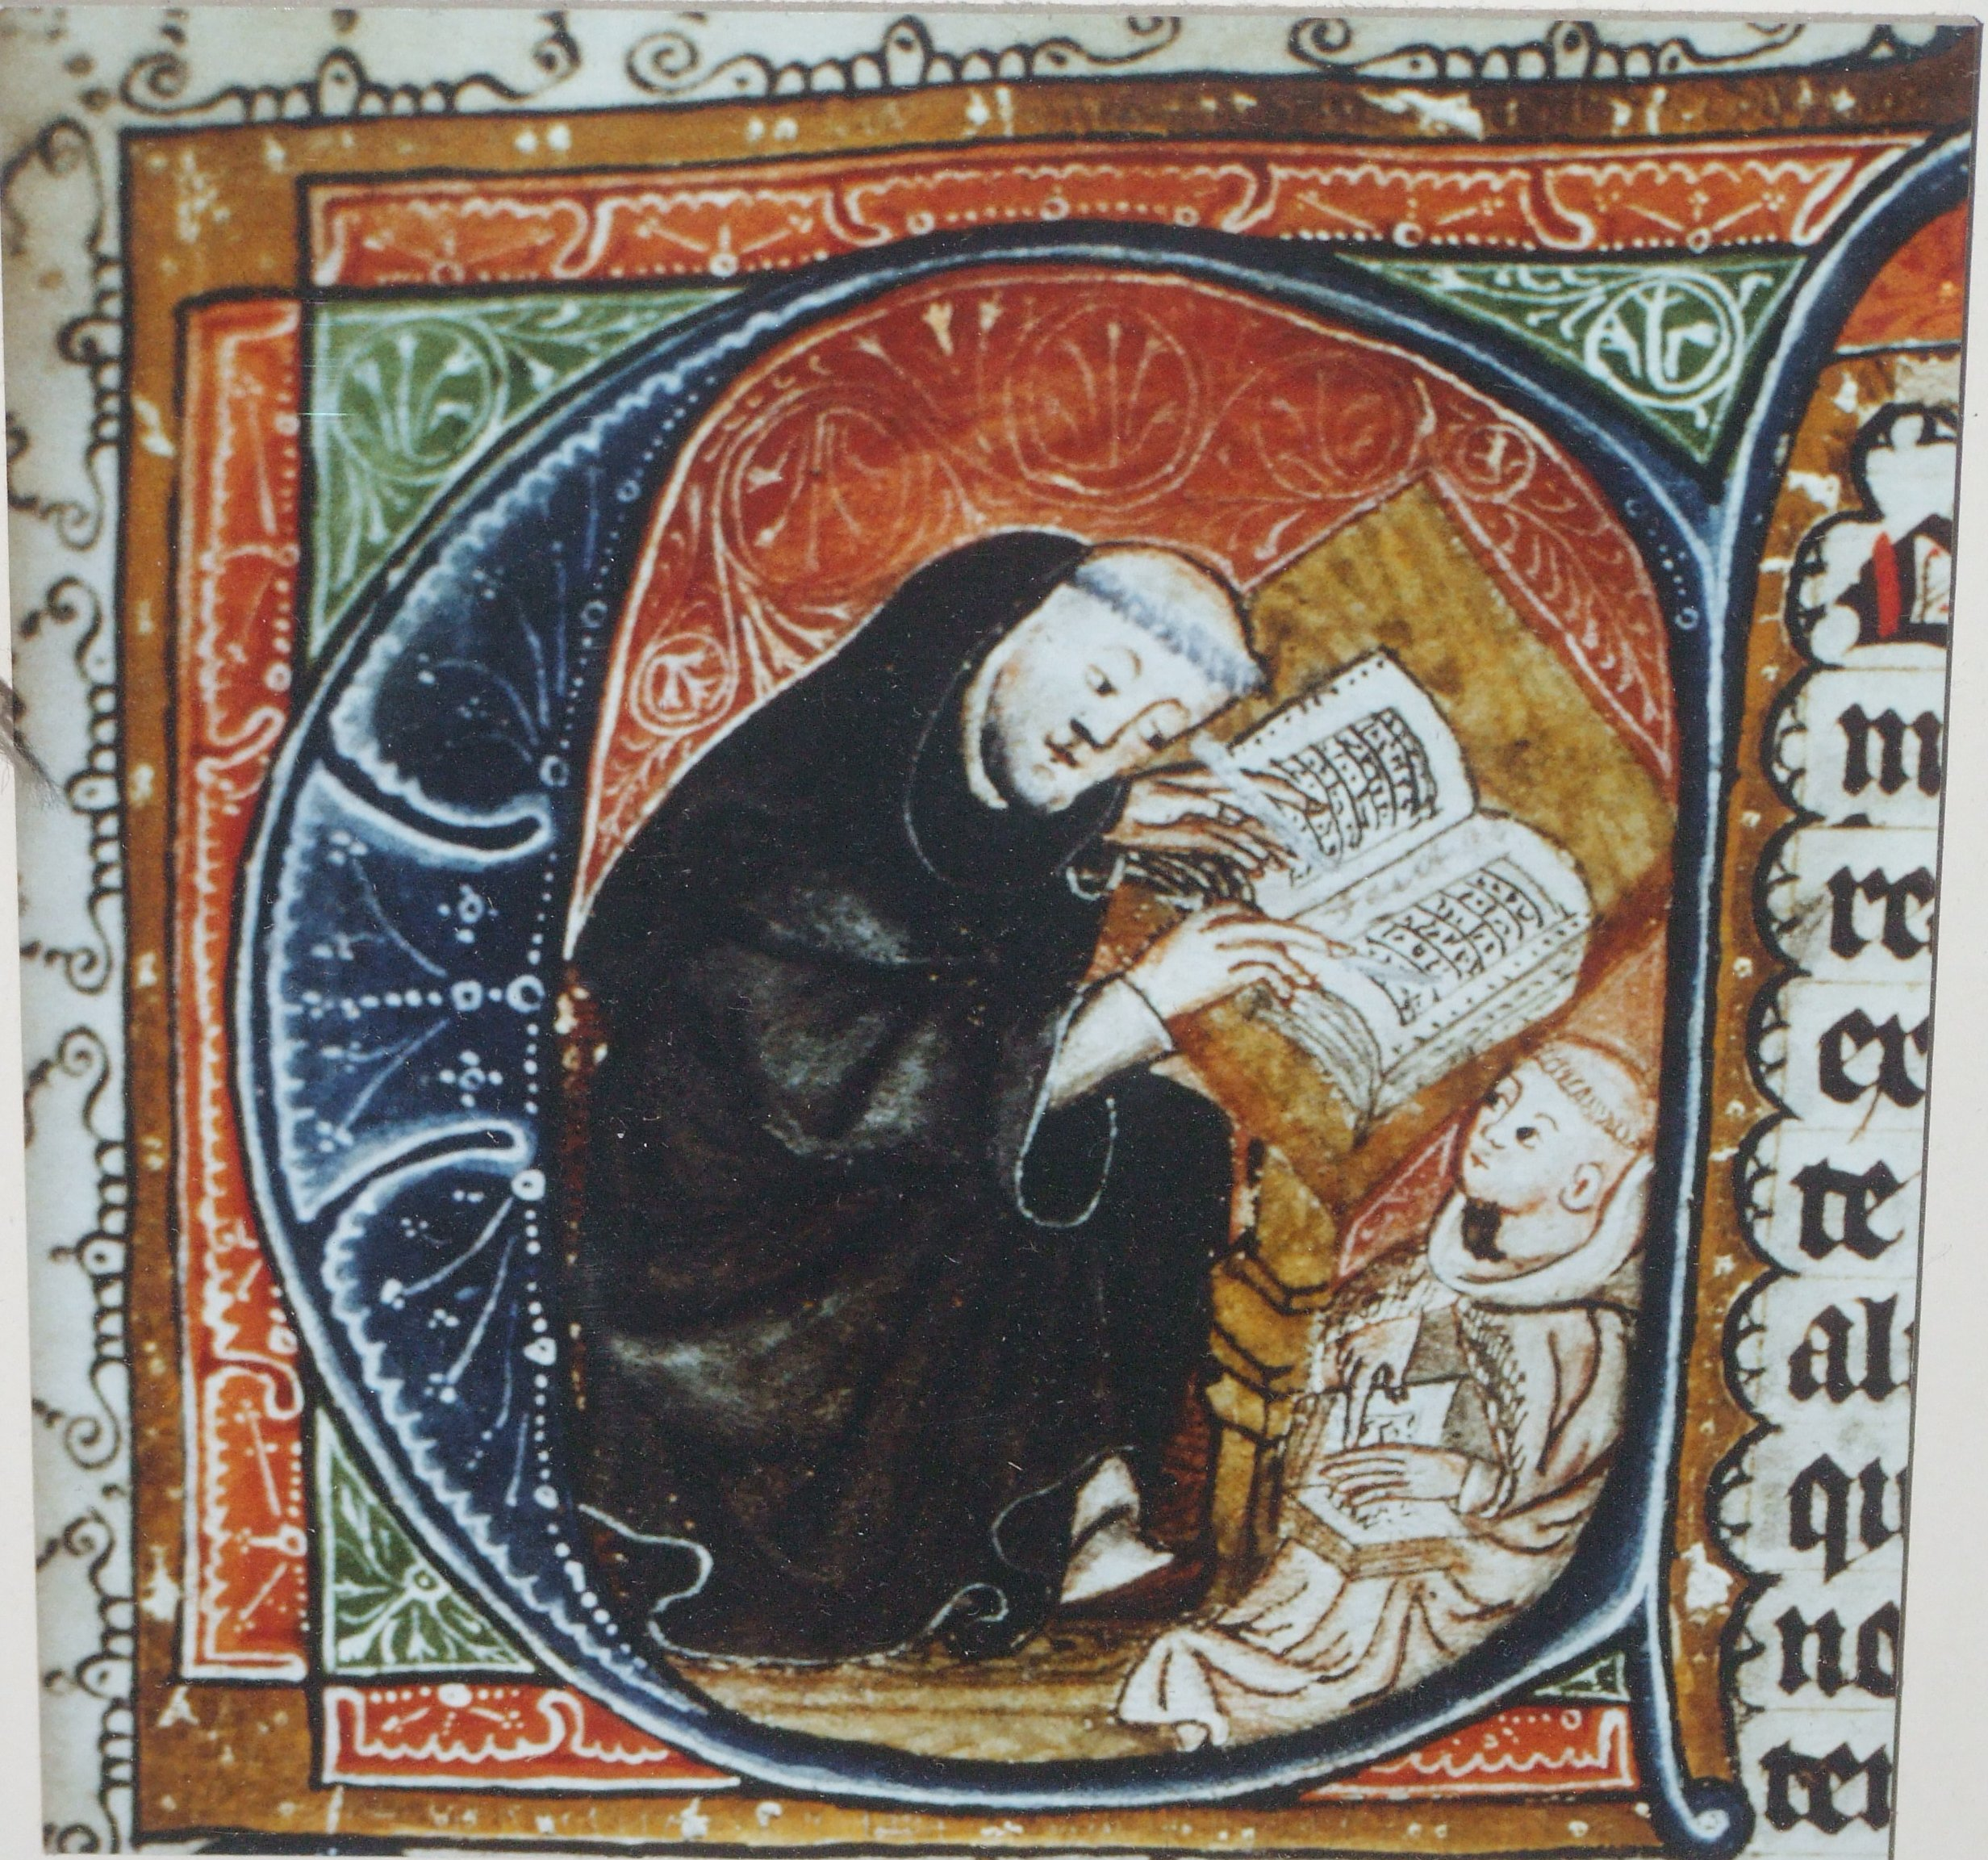
\includegraphics[width=20mm]{Caesarius_von_Heisterbach_als_Novizenmeister}
 \caption{Caesarius v. Heisterbach}
\end{marginfigure}
(inkl. Bildunterschrift) und Tabellen auf den Rand zu platzieren:

\begin{lstlisting}
 \begin{marginfigure}
 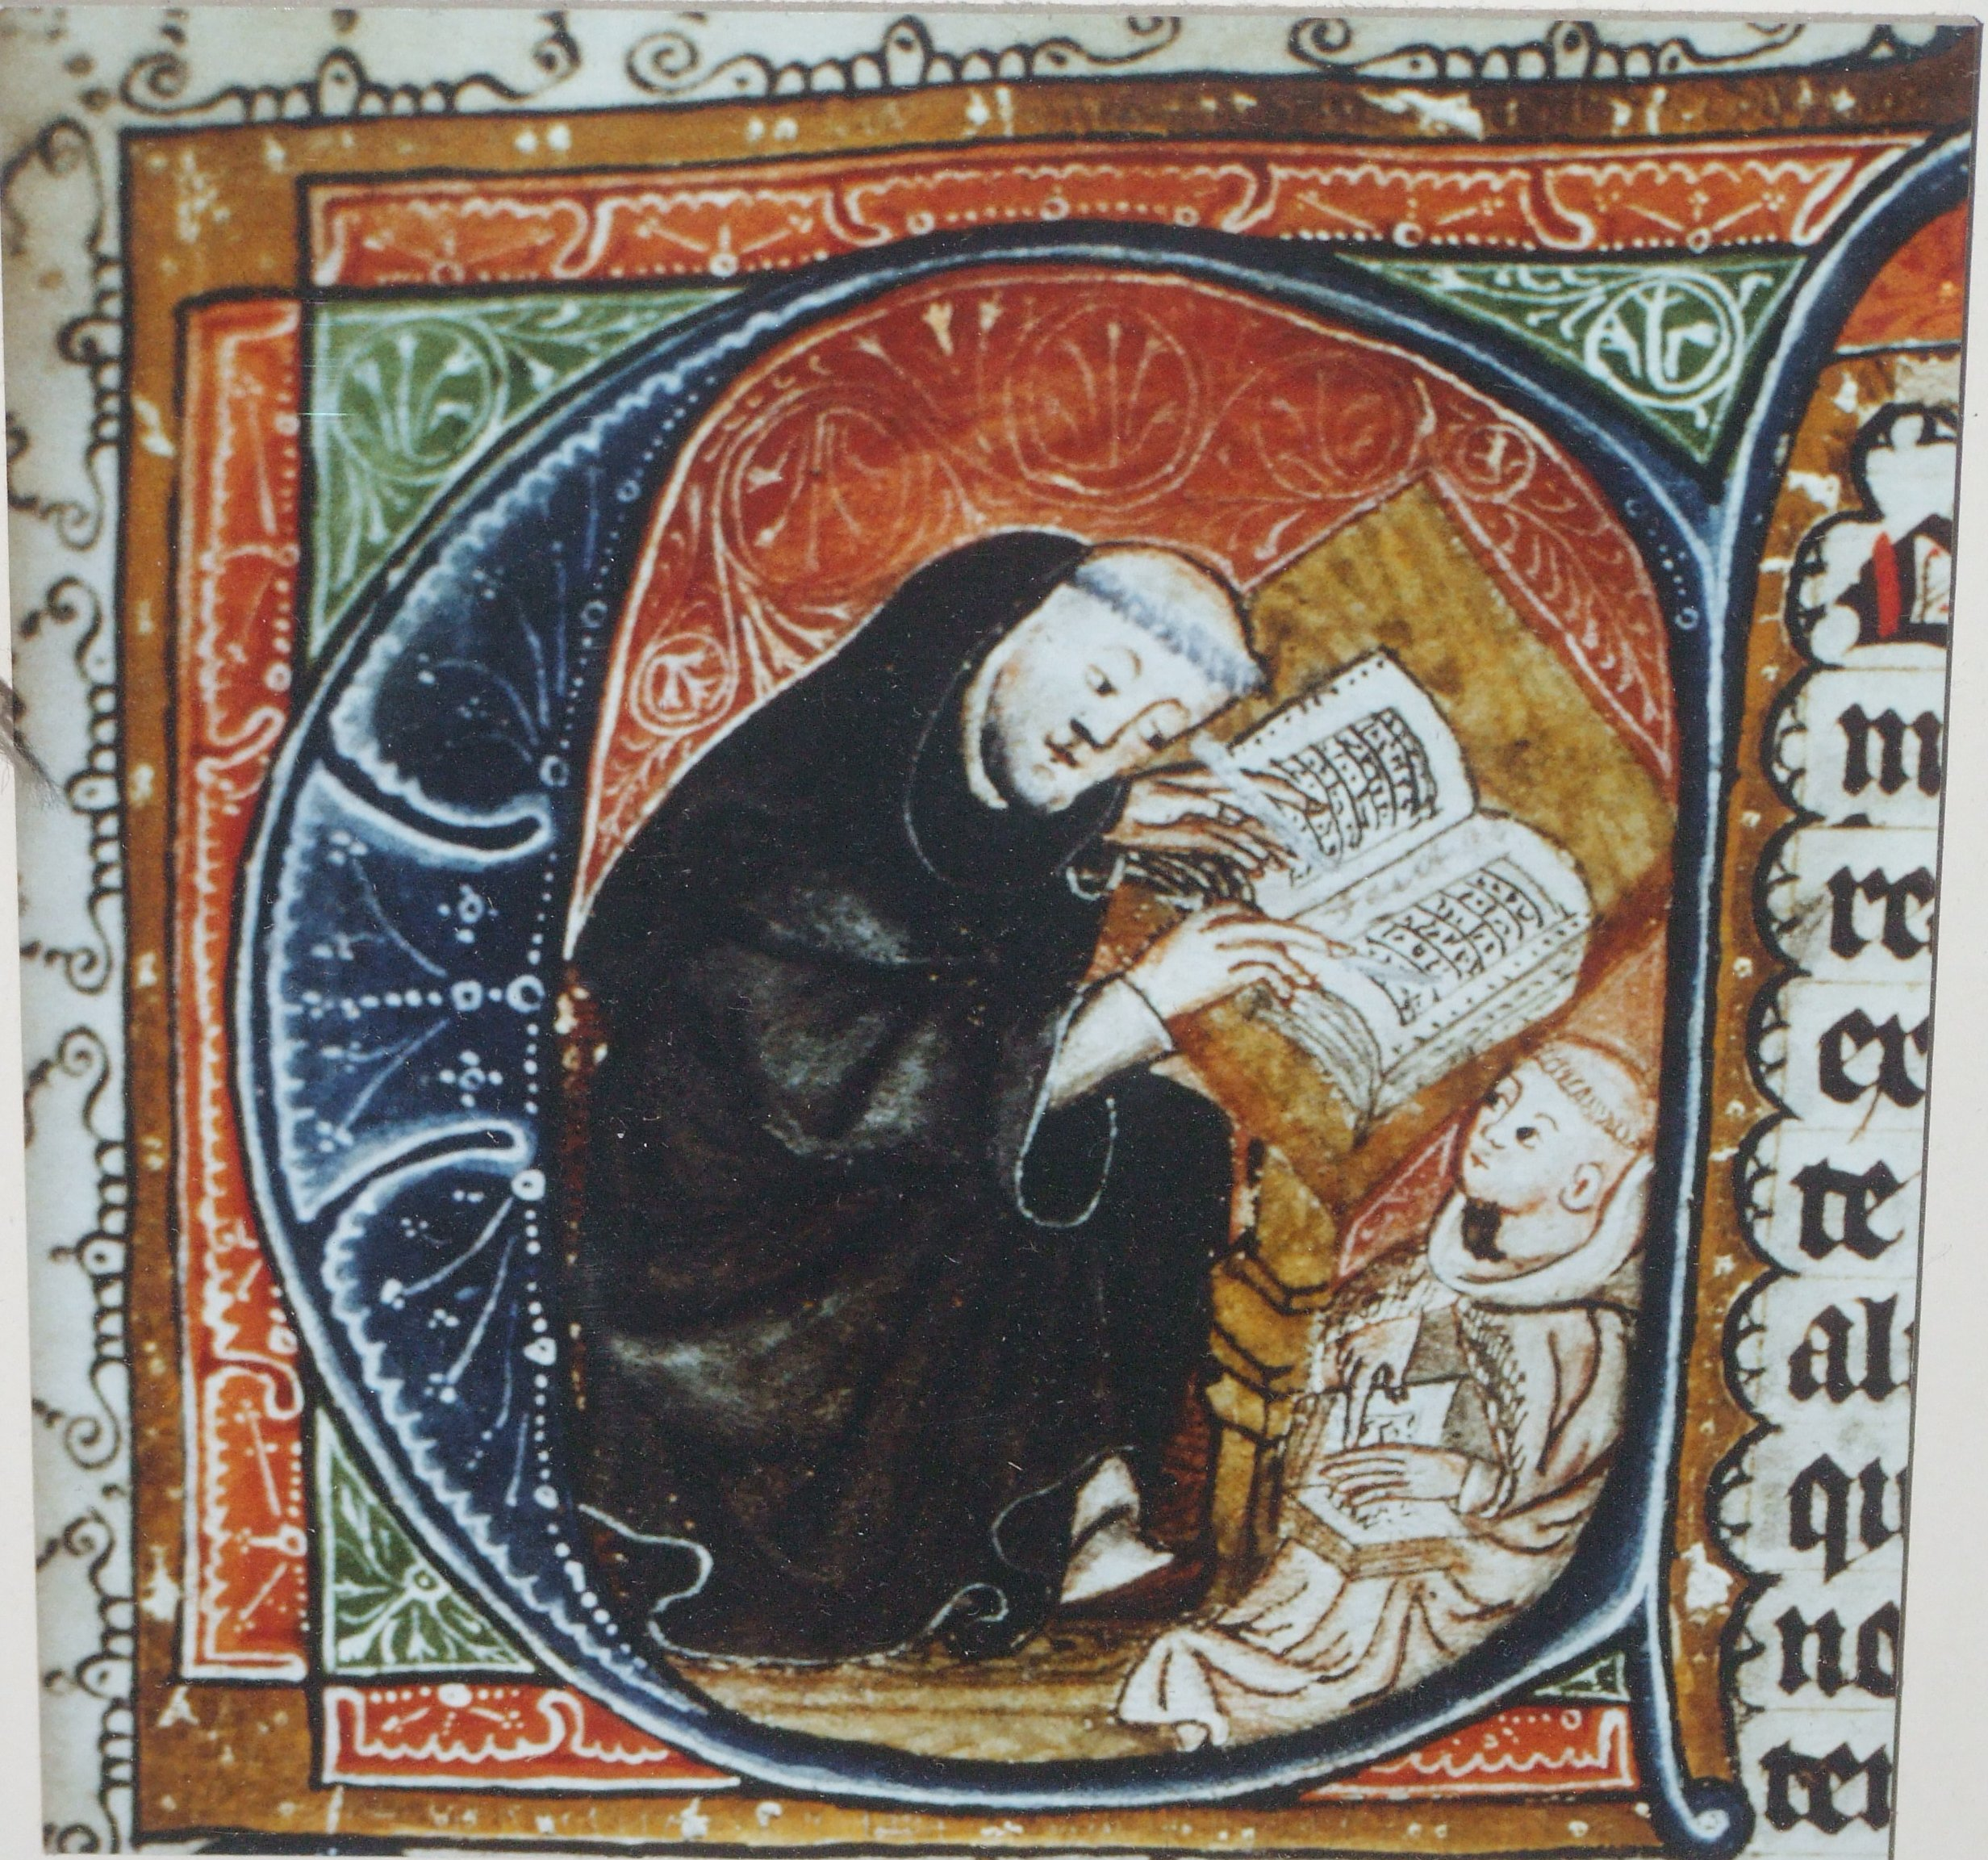
\includegraphics[width=20mm]{Caesarius_von_Heisterbach_als_Novizenmeister}
 \caption{Caesarius v. Heisterbach}
\end{marginfigure}
\end{lstlisting}


Eine weitere Option ist, die Beschriftung einer Gleitumgebung (Bild, Tabelle) auf den Rand zu
setzen, während die Gleitumgebung selbst die gesamte Breite des Textfeldes einnimmt.

Auch Bilder und Tabellen, die sich über die ganze Seitenbreite, d.\,h. den eigentlichen Satzspiegel
\emph{und} die Marginalspalte erstrecken, werden unterstützt.

Nähere Informationen enthält die Paketdokumentation.


\section{Texte mehrspaltig setzen}

Es gibt in \LaTeX{} zwei verschiedene Wege, zweispaltigen Satz zu erreichen:
Bereits der \LaTeX -Kern bietet die Möglichkeit, Texte zweispaltig zu setzen;
daneben gibt es das Paket \paket{multicol}, dass mehrspaltige Einschübe in einem ansonsten
einspaltigen Dokument ermöglicht.

Beide Verfahren haben ihre Berechtigung, denn es ergeben sich jeweils verschiedene
Vor- und Nachteile bzw. Einschränkungen:

\minisec{Das ganze Dokument zweispaltig setzen}

Wird als Dokumentklassen-Option \lstinline/twocolumn/ angegeben, wird das Dokument 
zweispaltig gesetzt. 
Der Titel mit Datum, Autorangabe, Abstract etc. werden als einspaltiger Kopf über beide 
Spalten gesetzt.


\minisec{Zweispaltige Einschübe in einem einspaltigen Dokument I: \LaTeX}

Daneben bietet \LaTeX die Möglichkeit, in einem Dokument eine zweispaltige Passage
zu integrieren. Die Passage wird mit dem Befehl \lstinline/\twocolumn[xxx] /
eingeleitet. Die angegebene Überschrift wird einspaltig über beide Spalten gesetzt.
Außer einer echten Überschrift (z.\,B. \lstinline/\section{}/ etc. sind hier auch
längere Einleitungstexte etc. möglich.

Mit dem Befehl \lstinline/\onecolumn/ wird wieder auf einspaltigen Satz zurückgestellt.

Beide Kommandos beginnen jeweils eine neue Seite, was ihre praktische Benutzbarkeit m.\,E.
stark einschränkt.


\minisec{Mehrspaltige Einschübe in einem einspaltigen Dokument II: \paket{multicol}}

\begin{multicols}{2}
 Die umfassendste Funktionalität bietet das Paket \paket{multicol} von Frank Mittelbach.
 Mit ihm lassen sich beliebige Textpassagen in mehreren Spalten in ein ansonsten
 einspaltiges Dokument einfügen.
 
 Der Beginn einer mehrspaltigen Passage wird durch \lstinline/\begin{multicols}{Zahl}/ 
 eingeleitet; die entsprechende Anweisung \lstinline/\end{multicols}/ schaltet wieder
 auf einspaltigen Satz um. \lstinline/Zahl/ steht dabei für die Anzahl der gewünschten 
 Spalten.                                            
\end{multicols}

\setlength{\columnseprule}{0.4pt}
\begin{multicols}{3}
 Dabei liegt es in der Veranwortung des Nutzers, nicht zuviele Spalten zu verlangen,
 da sonst die einzelnen Spalten zu schmal werden und sich Aussehen und Lesbarkeit erheblich
 verschlechtern.
 
 Faustregel: Der Wortabstand soll niemals größer sein als der Zeilenabstand.
 Evtl. kann es helfen, mehrspaltige Abschnitte im Flattersatz zu setzen.
 In typographischer Hinsicht ist dies ein sehr schlechter Absatz...
 
 Um dem Leser zu ermöglichen, die Spalten besser wahrzunehmen kann der Längenwert 
 \lstinline/columnseprule/ auf einen Wert größer 0 gestellt werden;
 in diesem Beispiel liegt er bei 0.4pt: \lstinline/\setlength{\columnseprule}{0.4pt}/.
 
 Daneben bietet das Paket weitere Einstellmöglichkeiten, wie. z.\,B. den Spaltenabstand
 oder die Farbe der Trennlinie.
\end{multicols}



\section{Das Konzept der \enquote{Gleitumgebung}}
\dictum[Heraklit?]{Alles fließt.}

\minisec{Gleitumgebungen beschriften: Das Paket \paket{caption}}

\section{Grafiken einbinden}

Voraussetzung: Paket \paket{graphicx} in Dokumentspräambel einbinden:
\lstinline/\usepackage{graphicx}/.

Dann fügt der Befehl \lstinline/\includegraphics[Optionen]{Name}/ an der jeweiligen Stelle
die angegebene Grafik (als eigenen Absatz) ein.
Als Option sollte z.\,B. die gewünschte Abbildungsgröße eingestellt werden.
Wieder sind sowohl absolute Angaben möglich als auch Bezugnahmen z.\,B. auf 
\lstinline/\textwidth/.

Meist möchte man die Abbibldung jedoch in eine Gleitumgebung einfügen, so dass das Satzprogramm
flexibler die Positionierung entscheiden kann (s. vorheriger Abschnitt).
Dazu dient die Umgebung \lstinline/figure/.
Dann ist auch die Angabe einer Bildunterschrift mit dem Paket \paket{caption} möglich.

Ggf. empfiehlt sich auch noch das Eibetten in eine \lstinline/center/-Umgebung,
um das Bild auf die Mitte des Satzspiegels zu zentrieren.

Alles zusammen sieht dann so aus:

\begin{lstlisting}
\begin{figure}
 \begin{center}
  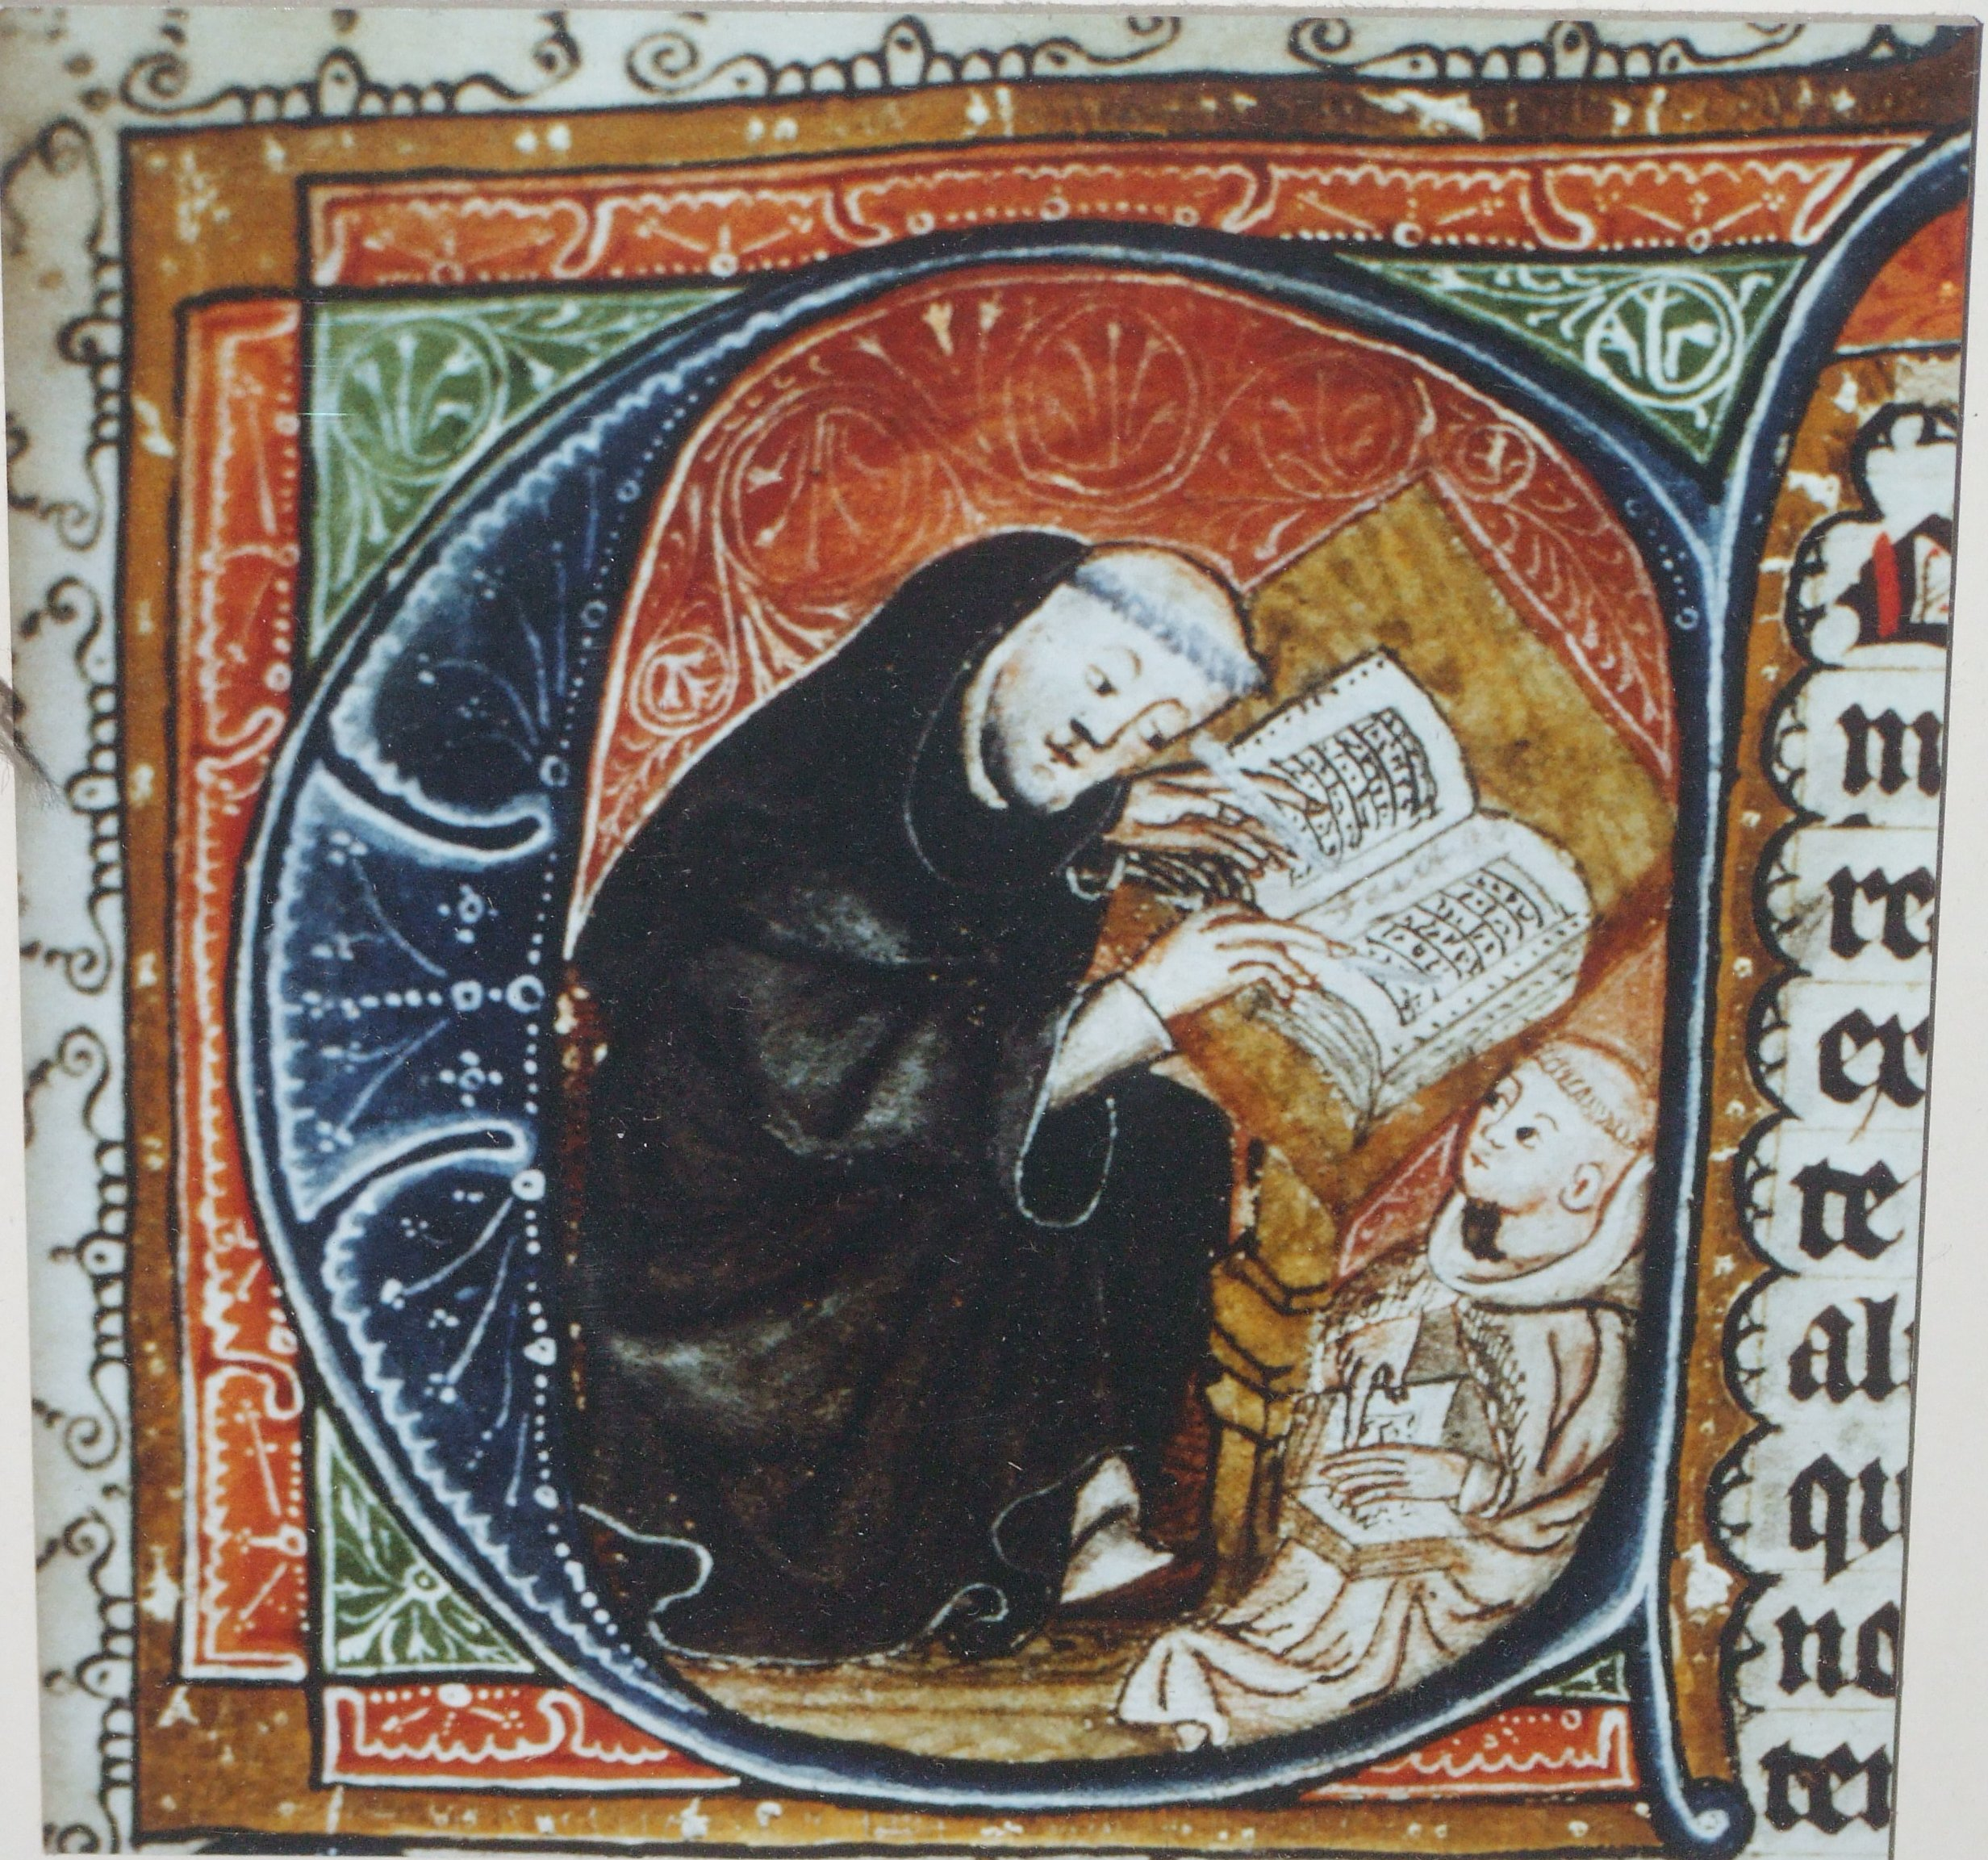
\includegraphics[width=.5\textwidth]{Caesarius_von_Heisterbach_als_Novizenmeister}
  \caption{Caesarius von Heisterbach als Novizenmeister}
 \end{center}
\end{figure} 
\end{lstlisting}


\begin{figure}[!htb]
\centering
  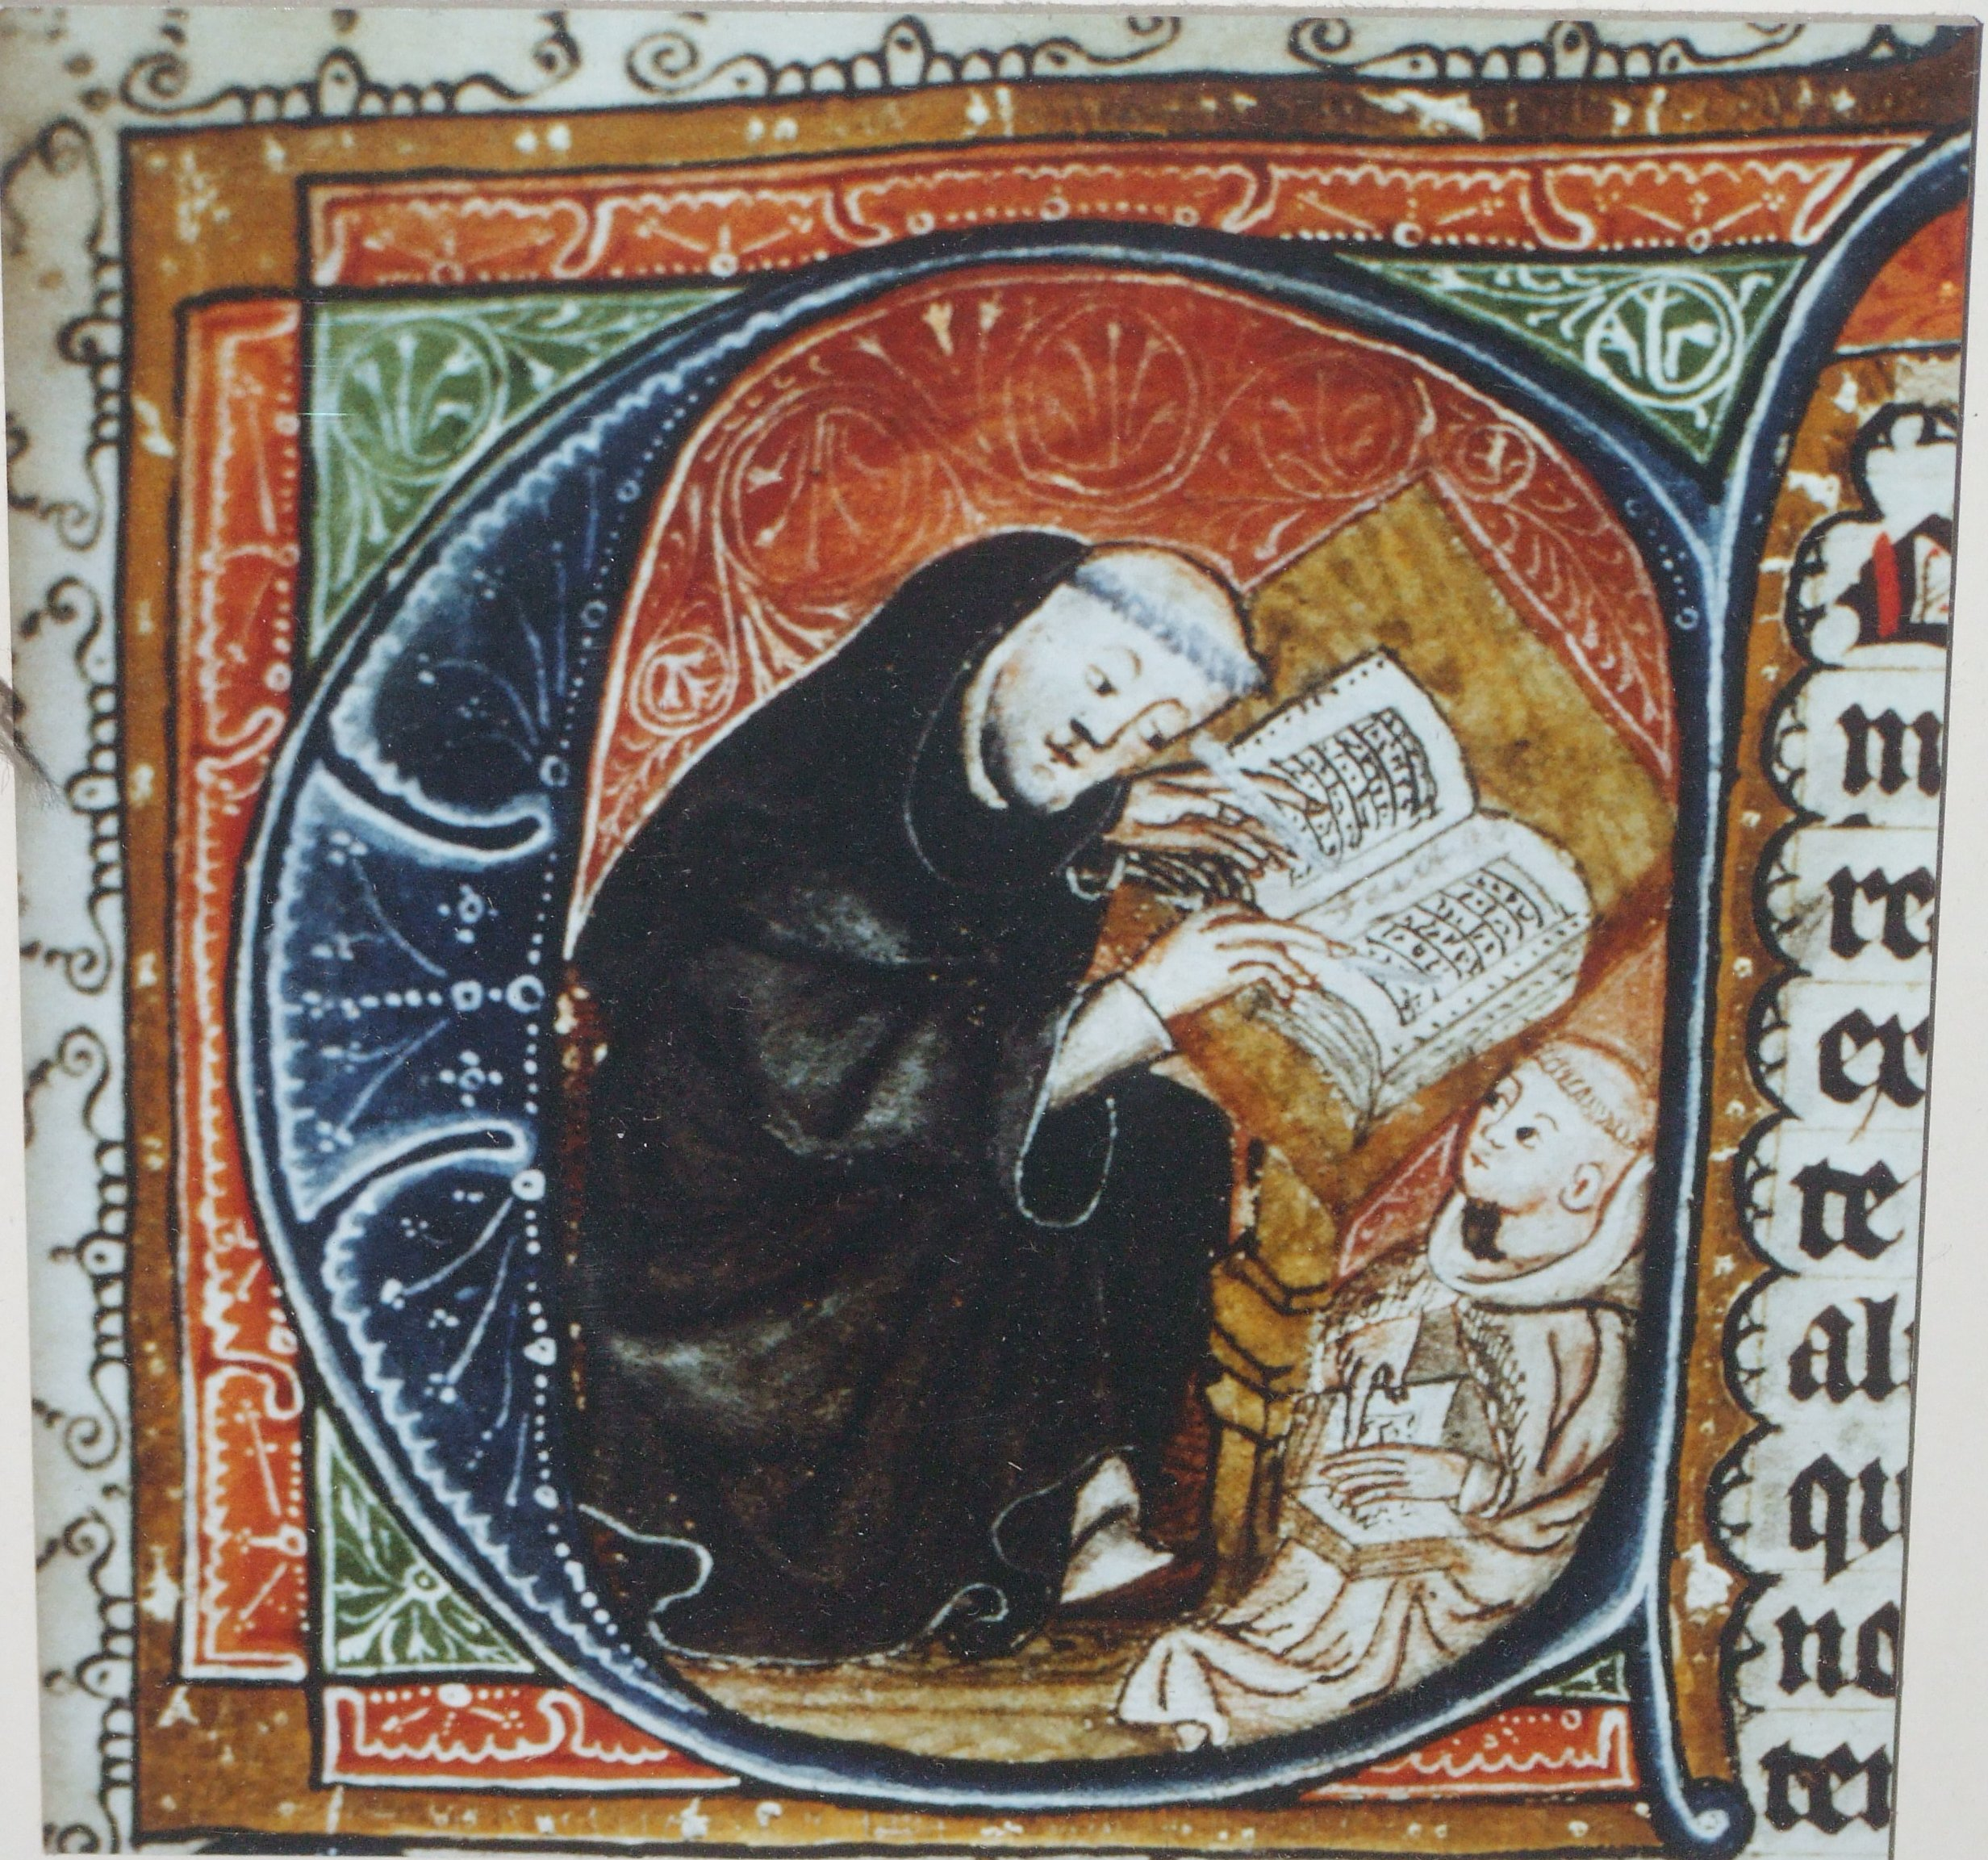
\includegraphics[width=.7\textwidth]{Caesarius_von_Heisterbach_als_Novizenmeister}
  \caption{Caesarius von Heisterbach als Novizenmeister}
\end{figure}

\section{Unter-Abbildungen mit \protect\paket{subcaption}}


\section{Diagramme zeichnen}
allgemeine vs. spezielle Lösungen

\subsection{Der unsaubere Weg: Open Office und co. benutzen}

Einbinden der fertigen Abb. als Grafik


\subsection{Die beiden wichtigsten Pakete: pstricks und tikz}

\minisec{pstricks}
\paket{pstricks}

\minisec{tikz}
\paket{tikz}

\subsection{Linguistische Strukturen}
\index{Linguistik} \index{x-bar-Schema} \index{Phrasenstruktur}
\paket{covington}
\footcite{roemer:dtk2008}
\footcite{roemer:dtk2016}


\minisec{Baumdiagramme}
\index{Baumdiagramm} \index{Stemma}

Das Paket \paket{forest} von Saso Zivanovic erlaubt einfache und sehr komplexe Baumsstrukturen:

\begin{LTXexample}
 \begin{forest}
  [VP
    [DP]
    [V'
      [V]
      [DP]
    ]
  ]
\end{forest}
\end{LTXexample}

\subsection{Ausgewählte Anwendungen}


\minisec{Zeitschienen}


\minisec{Stammbäume}


\minisec{Statistiken visualisieren}

Torten- und Balkendiagramme... 

\paket{datatool} ?



\section{Tabellen erstellen}

Komplexes Thema, Spezialliteratur gerechtfertigt.\footcite{voss:tabellen}


\paket{tabularx}

\paket{longtable}

\minisec{Tabellen drehen}
\index{Drehen von Texten}

\paket{rotatebox}


\section{Umgang mit Bibelstellen}
\index{Bibelstellen}

\paket{bibleref}

\paket{bibleref-german}

\paket{bibleref-parse}

Zur Registererstellung vgl. \fullref{Bibelstellenregister}.


\section{Lyrik-Satz}
\index{Gedicht} \index{Lyrik}

\paket{poemscol} (?) und andere?

\section{Dramen}
\paket{covington}
\paket{dramatist}
\footcite[xxx]{lesetypografie}


\section{Linmguistische Beispiele}

Mithilfe des Paketes \paket{gb4} lassen sich spezielle Bedürfnisse für Linguisten erfüllen: BLUPP


\section{Querverweise im Text}

%Philipp meint: Lukas hatte vorgeschlagen, zumindest /auch/ das cleveref-Paket hier vorzustellen, das nimmt einem etwas Arbeit ab

\lstinline/\label{key}/

\lstinline/\ref{key}/

\lstinline/\pageref{key}/


\section{Eigene Kommandos und Umgebungen definieren}
\label{makros}

\minisec{Kommandos}

\minisec{Umgebungen}
